% Options for packages loaded elsewhere
\PassOptionsToPackage{unicode}{hyperref}
\PassOptionsToPackage{hyphens}{url}
%
\documentclass[
]{book}
\usepackage{lmodern}
\usepackage{amssymb,amsmath}
\usepackage{ifxetex,ifluatex}
\ifnum 0\ifxetex 1\fi\ifluatex 1\fi=0 % if pdftex
  \usepackage[T1]{fontenc}
  \usepackage[utf8]{inputenc}
  \usepackage{textcomp} % provide euro and other symbols
\else % if luatex or xetex
  \usepackage{unicode-math}
  \defaultfontfeatures{Scale=MatchLowercase}
  \defaultfontfeatures[\rmfamily]{Ligatures=TeX,Scale=1}
\fi
% Use upquote if available, for straight quotes in verbatim environments
\IfFileExists{upquote.sty}{\usepackage{upquote}}{}
\IfFileExists{microtype.sty}{% use microtype if available
  \usepackage[]{microtype}
  \UseMicrotypeSet[protrusion]{basicmath} % disable protrusion for tt fonts
}{}
\makeatletter
\@ifundefined{KOMAClassName}{% if non-KOMA class
  \IfFileExists{parskip.sty}{%
    \usepackage{parskip}
  }{% else
    \setlength{\parindent}{0pt}
    \setlength{\parskip}{6pt plus 2pt minus 1pt}}
}{% if KOMA class
  \KOMAoptions{parskip=half}}
\makeatother
\usepackage{xcolor}
\IfFileExists{xurl.sty}{\usepackage{xurl}}{} % add URL line breaks if available
\IfFileExists{bookmark.sty}{\usepackage{bookmark}}{\usepackage{hyperref}}
\hypersetup{
  pdftitle={Topology Inference for Radial Distribution Feeder based on Power Flow},
  pdfauthor={Jie Xu (s181238)},
  hidelinks,
  pdfcreator={LaTeX via pandoc}}
\urlstyle{same} % disable monospaced font for URLs
\usepackage{longtable,booktabs}
% Correct order of tables after \paragraph or \subparagraph
\usepackage{etoolbox}
\makeatletter
\patchcmd\longtable{\par}{\if@noskipsec\mbox{}\fi\par}{}{}
\makeatother
% Allow footnotes in longtable head/foot
\IfFileExists{footnotehyper.sty}{\usepackage{footnotehyper}}{\usepackage{footnote}}
\makesavenoteenv{longtable}
\usepackage{graphicx}
\makeatletter
\def\maxwidth{\ifdim\Gin@nat@width>\linewidth\linewidth\else\Gin@nat@width\fi}
\def\maxheight{\ifdim\Gin@nat@height>\textheight\textheight\else\Gin@nat@height\fi}
\makeatother
% Scale images if necessary, so that they will not overflow the page
% margins by default, and it is still possible to overwrite the defaults
% using explicit options in \includegraphics[width, height, ...]{}
\setkeys{Gin}{width=\maxwidth,height=\maxheight,keepaspectratio}
% Set default figure placement to htbp
\makeatletter
\def\fps@figure{htbp}
\makeatother
\setlength{\emergencystretch}{3em} % prevent overfull lines
\providecommand{\tightlist}{%
  \setlength{\itemsep}{0pt}\setlength{\parskip}{0pt}}
\setcounter{secnumdepth}{5}
\usepackage{booktabs}
\usepackage{amsthm}
\makeatletter
\def\thm@space@setup{%
  \thm@preskip=8pt plus 2pt minus 4pt
  \thm@postskip=\thm@preskip
}
\makeatother
\usepackage{booktabs}
\usepackage{longtable}
\usepackage{array}
\usepackage{multirow}
\usepackage{wrapfig}
\usepackage{float}
\usepackage{colortbl}
\usepackage{pdflscape}
\usepackage{tabu}
\usepackage{threeparttable}
\usepackage{threeparttablex}
\usepackage[normalem]{ulem}
\usepackage{makecell}
\usepackage{xcolor}
\usepackage[]{natbib}
\bibliographystyle{apalike}

\title{Topology Inference for Radial Distribution Feeder based on Power Flow}
\author{Jie Xu (s181238)}
\date{2020-12-14}

\begin{document}
\maketitle

{
\setcounter{tocdepth}{1}
\tableofcontents
}
\hypertarget{introduction}{%
\chapter{Introduction}\label{introduction}}

This website hosts slides for defence of my master graduation project in the
Department of Electrical Engineering at Technical University of Denmark. How
households are connected to distribution network is always unknown. A framework
to infer such connections by utilising all kinds of information is proposed in
this project.

\hypertarget{problem-setting}{%
\subsection*{Problem Setting}\label{problem-setting}}
\addcontentsline{toc}{subsection}{Problem Setting}

\begin{quote}
How households are connected to distribution network is usually unknown.
\end{quote}

Available information for topology inference:

\begin{quote}
There are three kinds of available information in this project.
\end{quote}

\begin{itemize}
\tightlist
\item
  geographical information about buses
\item
  voltage magnitudes of all the phases of all the buses
\item
  some real power injection profiles
\end{itemize}

\begin{quote}
For example, where they are located and barriers between them.
There is no literature mentioning how to handle geographical information.
\end{quote}

Association network inference:

\begin{quote}
In the literature, a technique called association network inference is
usually used. Correlation between entities are derived based on some entity
attributes. The face that number of edges in a mathematical tree is always 1
less than number of entities makes the problem simpler.
\end{quote}

\begin{itemize}
\tightlist
\item
  Correlation between entities.
\item
  \(|\mathcal{E}| = |\mathcal{N}| - 1\)
\end{itemize}

\begin{quote}
However, there are two reasons why such technique cannot be used here.
\end{quote}

\begin{itemize}
\tightlist
\item
  Spurious correlation resulted from correlated profiles.
\item
  Missing entity attribute.
\end{itemize}

\begin{quote}
The second reason will be discussed in detail later.
\end{quote}

\hypertarget{flowchart}{%
\subsection*{Flowchart}\label{flowchart}}
\addcontentsline{toc}{subsection}{Flowchart}

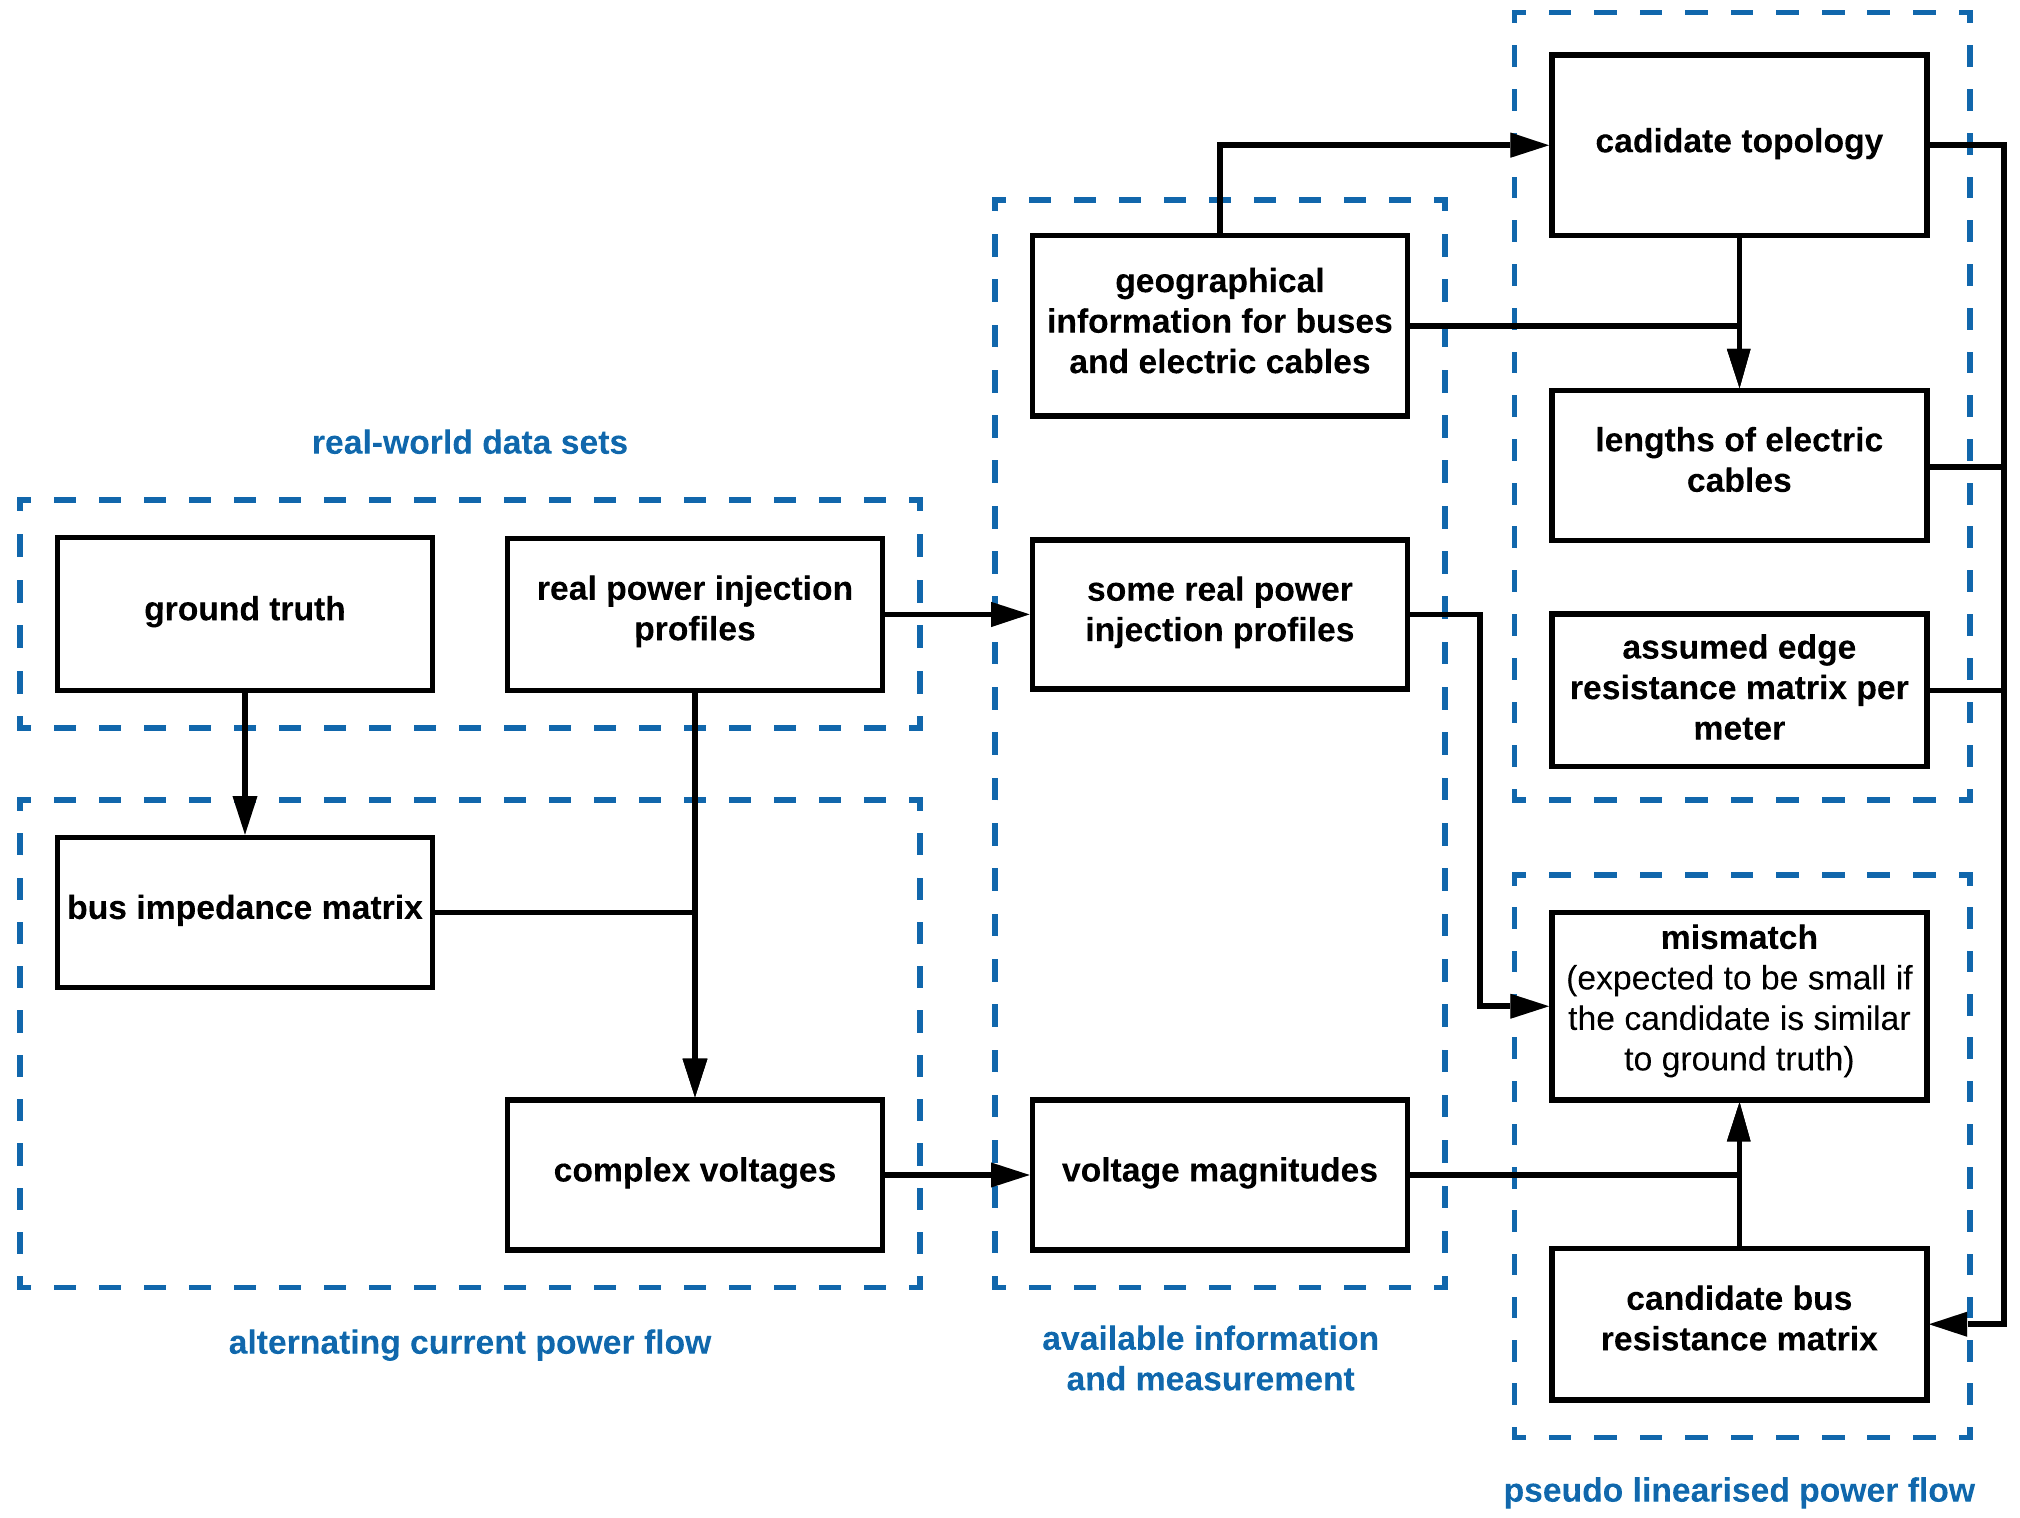
\includegraphics{Pictures/figFlowchart3.png}

\begin{quote}
There are three columns. In the left column, ground truth, the true topology,
is known, and used to simulate available measurement using power flow
program. Three boxes in the middle represents three kinds of information
disucssed before. Note that ground truth is not known and we want to find it.
Programs in the right column are used to make inference about the topology.
\end{quote}

\textbf{Ground truth} is not known, but used to simulate available measurement.

Two batches of computer programs:

\begin{itemize}
\tightlist
\item
  power flow
\item
  three algorithms to handle directed graphs
\end{itemize}

\begin{quote}
The second batch will not be discussed in detail.
\end{quote}

\hypertarget{radial-distribution-feeder}{%
\chapter{Radial Distribution Feeder}\label{radial-distribution-feeder}}

\begin{quote}
Essential concepts are discussed in following three parts.
\end{quote}

\begin{itemize}
\tightlist
\item
  bus and edge, \protect\hyperlink{bus-edge}{-\textgreater{} 2.1}
\item
  two special concepts for power flow, \protect\hyperlink{concepts}{-\textgreater{} 2.2}
\item
  case with 70 buses, \protect\hyperlink{case}{-\textgreater{} 2.3}
\end{itemize}

\hypertarget{bus-edge}{%
\section{Bus and Edge}\label{bus-edge}}

\begin{quote}
Power grids can be roughly described here by following three concepts.
\end{quote}

\begin{table}[H]
\centering
\begin{tabular}[t]{l|l|l}
\hline
type & definition & examples\\
\hline
edge & transport power from one place to another & cable, transformer, capacitor\\
\hline
conversion element & convert power from or to another form & solar panel, battery\\
\hline
bus & where two edges joint or end of an edge & slack bus, PQ bus, PV bus\\
\hline
\end{tabular}
\end{table}

\begin{quote}
Only one type of edge, cable, is considered. The method applies when there
are transformers, capacitors, and other devices. Usually, there is one slack
bus in distribution network and is referred to as root here.
\end{quote}

\begin{itemize}
\tightlist
\item
  Ignore conversion elements. Not necessary in power flow calculation.
\item
  Cable.
\item
  One slack bus -\textgreater{} \textbf{root}.
\end{itemize}

\begin{center}\rule{0.5\linewidth}{0.5pt}\end{center}

Impedance of cable is proportional to its length.

Unit impedance matrix for case-70:
\[ \begin{aligned}
  \boldsymbol{\bar{Z}}_{a b c}
  =
  \left[\begin{array}{lll}
    0.000412+1.558e^{-4} j
    & 0.000206+7.791e^{-5} j
    & 0.000206+7.791e^{-5} j \\
    0.000206+7.791e^{-5} j
    & 0.000412+1.558e^{-4} j
    & 0.000206+7.791e^{-5} j \\
    0.000206+7.791e^{-5} j
    & 0.000206+7.791e^{-5} j
    & 0.000412+1.558e^{-4}j
  \end{array}\right]
  \nonumber
\end{aligned} \]

\begin{quote}
It is assumed that there is only one type of cable in case-70, and its
impedance matrix for one-meter-long cable is known. Diagonal values are the
same, and two times of off-diagonal values. So it is sufficient to store this
matrix with one number for resistance and one number for reactance.
\end{quote}

\hypertarget{concepts}{%
\section{Two Special Concepts}\label{concepts}}

Essential for power flow calculation.

\begin{quote}
Such two concepts cannot be found in the literature, but are essential for
power flow when taking multiple phases into account.
\end{quote}

\hypertarget{channel}{%
\subsection*{Channel}\label{channel}}
\addcontentsline{toc}{subsection}{Channel}

\begin{itemize}
\tightlist
\item
  \textbf{channel}: refer to one phase in some bus
\item
  \textbf{active channel}: there are non-zero injections (connected to some
  conversion element)
\item
  \textbf{observed active channel}: such non-zero injections are known
\end{itemize}

It is assumed that all inactive channels are observed.

\begin{quote}
That is, it is known that there is no power injection at those channels.
\end{quote}

\hypertarget{snapshot}{%
\subsection*{Snapshot}\label{snapshot}}
\addcontentsline{toc}{subsection}{Snapshot}

\textbf{Snapshot}: include power injections and voltages at one time index

\begin{itemize}
\tightlist
\item
  Duration is 1 s in this project.
\end{itemize}

\textbf{Zero‐load snapshot} : when power injections at all the channels are zero

\begin{quote}
Such two symbols will be used later.
\end{quote}

\begin{itemize}
\tightlist
\item
  \(\boldsymbol{\bar{V}}_\text{zero}\): voltages in zero‐load snapshot
\item
  \(V_\text{rate}\): rated voltage magnitude, 230 V
\end{itemize}

\hypertarget{case}{%
\section{Case with 70 Buses}\label{case}}

\begin{quote}
To make the project manageable:
\end{quote}

Assumptions about feeders:

\begin{itemize}
\tightlist
\item
  one path to any bus (tree)
\item
  one step-down transformer
\item
  rated voltage, 230 V
\item
  three-phase four-wire cable
\item
  one phase star connection
\end{itemize}

\begin{center}\rule{0.5\linewidth}{0.5pt}\end{center}

A case with 70 buses is primarily used here:

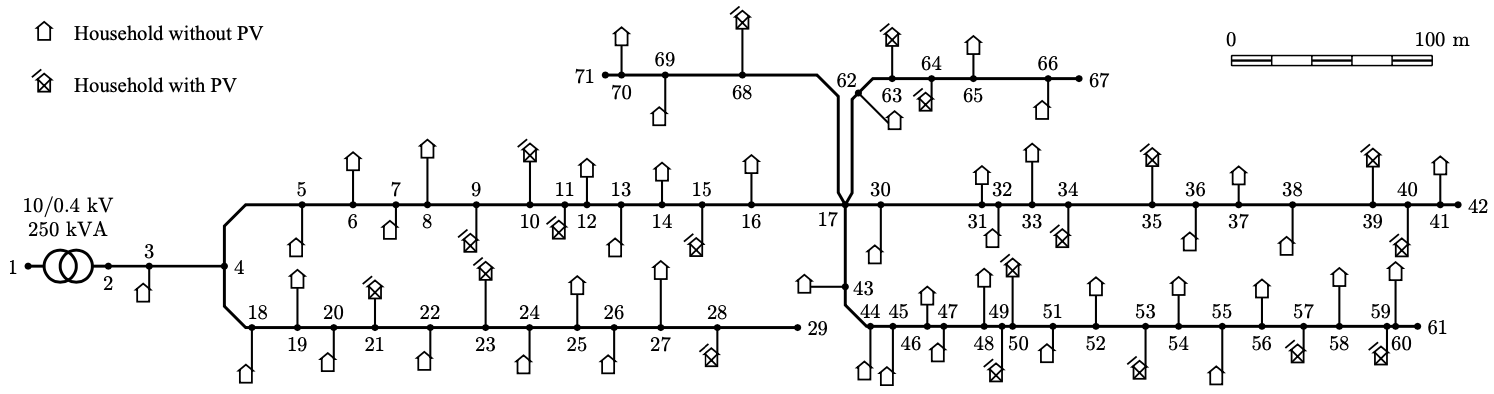
\includegraphics{Pictures/case70true.png}

\begin{itemize}
\tightlist
\item
  located in Belgium
\item
  bus 1 is omitted
\item
  70 buses
\item
  207 channels
\end{itemize}

\hypertarget{problem-formulation}{%
\chapter{Problem Formulation}\label{problem-formulation}}

\begin{itemize}
\tightlist
\item
  information in a directed graph \href{directed}{-\textgreater{} 3.1}
\item
  integer programming formulation \protect\hyperlink{IP}{-\textgreater{} 3.3}
\item
  local search heuristic algorithm \protect\hyperlink{combinatorial}{-\textgreater{} 3.4}
\end{itemize}

\begin{center}\rule{0.5\linewidth}{0.5pt}\end{center}

\begin{quote}
There is an issue here that I will discuss after a summary in the end.
\end{quote}

\begin{itemize}
\tightlist
\item
  remove overlapping edge \protect\hyperlink{overlapping}{-\textgreater{} 3.2}
\end{itemize}

\hypertarget{directed}{%
\section{Directed Graph}\label{directed}}

\begin{quote}
All the information can be stored in a weighted directed graph.
\end{quote}

\textbf{weighted directed graph}
\(G = (\mathcal{N}, \mathcal{E}, \sigma, \tau, \omega)\)

\begin{itemize}
\tightlist
\item
  set of nodes: \(\mathcal{N}\)
\item
  set of edges: \(\mathcal{E}\)
\item
  incidence functions: source \(\sigma\), target \(\tau\)
\item
  (edge) weighting function, \(\omega: \mathcal{E} \rightarrow \mathbb{R}\).
\end{itemize}

\textbf{complete graph for a set of nodes}

\begin{itemize}
\tightlist
\item
  all edges are \textbf{potential edges}
\item
  some are impossible to exist
\item
  possible to derive their lengths
\item
  2-D Euclidean distance as weight
\item
  \emph{association network inference cannot be used}
\end{itemize}

\textbf{spanning arborescence (SA)}

\begin{itemize}
\tightlist
\item
  subgraph of a directed graph
\item
  root
\item
  include every bus
\end{itemize}

\textbf{feasible region}

\begin{itemize}
\tightlist
\item
  All the SAs.
\item
  Number of SA is finite, making it a \protect\hyperlink{combinatorial}{combinatorial
  optimisation problem}.
\item
  Count number of SA.
\end{itemize}

\hypertarget{overlapping}{%
\section{Remove Overlapping Edge}\label{overlapping}}

For example, in case-70:

\[
\begin{array}{lllll}
  \hline
  \textbf{shortest path} & <
  & \textbf{direct edge} & \times \textbf{threshold}
  & \text{-> } \textbf{remove direct edge} \\
  \hline
  \text{"b17‐b43-b29"} & < & \text{"b17-b29"} & \times 1.1
  & \text{-> remove "b17-b29"} \\
  \text{"b44‐b43-b29"} & > & \text{"b44-b29"} & \times 1.1
  & \text{-> keep "b44-b29"} \\
  \hline
\end{array}
\]

\begin{center}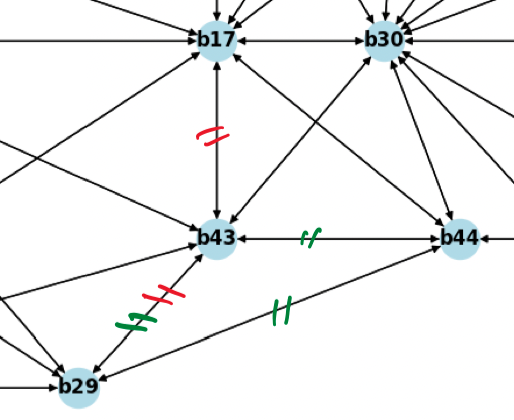
\includegraphics[width=0.7\linewidth]{Pictures/overlapGeth} \end{center}

However:

\begin{itemize}
\tightlist
\item
  446 possible potential edges
\item
  over \(10^{45}\) spanning arborescences
\end{itemize}

\protect\hyperlink{summary}{-\textgreater{} summary}

\hypertarget{IP}{%
\section{Integer Programming}\label{IP}}

Sets:

\[
\begin{array}{ll}
  \hline
  \textbf{symbol} & \textbf{definition} \\
  \hline
  \mathcal{E}
  & \text{all the potential edges (edges in the complete graph)} \\
  \mathcal{C}
  & \text{available measurements of voltages and power injections} \\
  \mathcal{E}_\text{impossible}
  & \text{potential edges that are impossible to exist} \\
  \hline
\end{array}
\]

Variables:

\[
\begin{array}{llll}
  \hline
  \textbf{symbol} & \textbf{definition} & \textbf{type} & \textbf{set} \\
  \hline
  x_{i j} & \text{if edge from i to j is in the solution}
  & \{0, 1\} & \mathcal{E} \\
  \hline
\end{array}
\]

Constants:

\[
\begin{array}{lll}
  \hline
  \textbf{symbol} & \textbf{definition} & \textbf{set} \\
  \hline
  d_{i, j} & \text{Euclidean distance from i to j}
  & \mathcal{E} \\
  \hline
\end{array}
\]

\begin{center}\rule{0.5\linewidth}{0.5pt}\end{center}

\[
\begin{aligned}
  \min_{x_{i j} \forall (i, j) \in \mathcal{E}} \quad
    & (1 - \alpha) \sum_{(i, j) \in \mathcal{E}} d_{i j} x_{i j}
    + \alpha \mathcal{H}
    \left(\{x_{i j} \forall (i, j) \in \mathcal{E} \}, \mathcal{C} \right) \\
  \text{s.t.} \quad & \sum_{(i, j) \in \delta^{-}(j)} x_{i j} = 1
    \quad \forall j \in V^{\prime}
    \quad \text{(a directed forest)} \\
  & \sum_{(i, j) \in \delta^{-}(S)} x_{i j} \geq 1
    \quad \forall S \subseteq V^{\prime},|S| \geq 2
    \quad \text{(a connected graph)} \\
  & x_{i j} = 0
    \quad \forall (i, j) \in \mathcal{E}_\text{impossible}
    \quad \text{(remove impossible potential edges)}
\end{aligned}
\]

Two terms in the objective function:

\[
\begin{array}{lll}
  \hline
  \textbf{term} & \textbf{definition} & \textbf{coefficient} \\
  \hline
  (1 - \alpha) \sum_{(i, j) \in \mathcal{E}} d_{i j} x_{i j}
  & \text{weight of candidate arborescence}
  & 1 - \alpha \\
  \alpha \mathcal{H}
  \left(\{x_{i j} \forall (i, j) \in \mathcal{E} \}, \mathcal{C} \right)
  & \text{assessment of candidate arborescence}
  & \alpha \\
  \hline
\end{array}
\]

Three sets of constraints:

\begin{itemize}
\tightlist
\item
  First two sets ensure arborescence. \citep{fischetti1997branch}
\item
  Last set removes impossible potential edges.
\end{itemize}

\hypertarget{combinatorial}{%
\section{Local Search}\label{combinatorial}}

At least two possible values for \(\alpha\):

\[
\begin{array}{llll}
  \hline
  \textbf{value} & \textbf{term lefted} & \textbf{to find}
  & \textbf{disadvantage} \\
  \hline
  1
  & \mathcal{H}
  \left(\{x_{i j} \forall (i, j) \in \mathcal{E} \}, \mathcal{C} \right)
  & \text{ground truth}
  & \text{NP-hard and non-linear} \\
  0
  & \sum_{(i, j) \in \mathcal{E}} d_{i j} x_{i j}
  & \text{topology with min total cable length}
  & \text{cannot find ground truth} \\
  \hline
\end{array}
\]

Such two situations can be visualised:

\begin{center}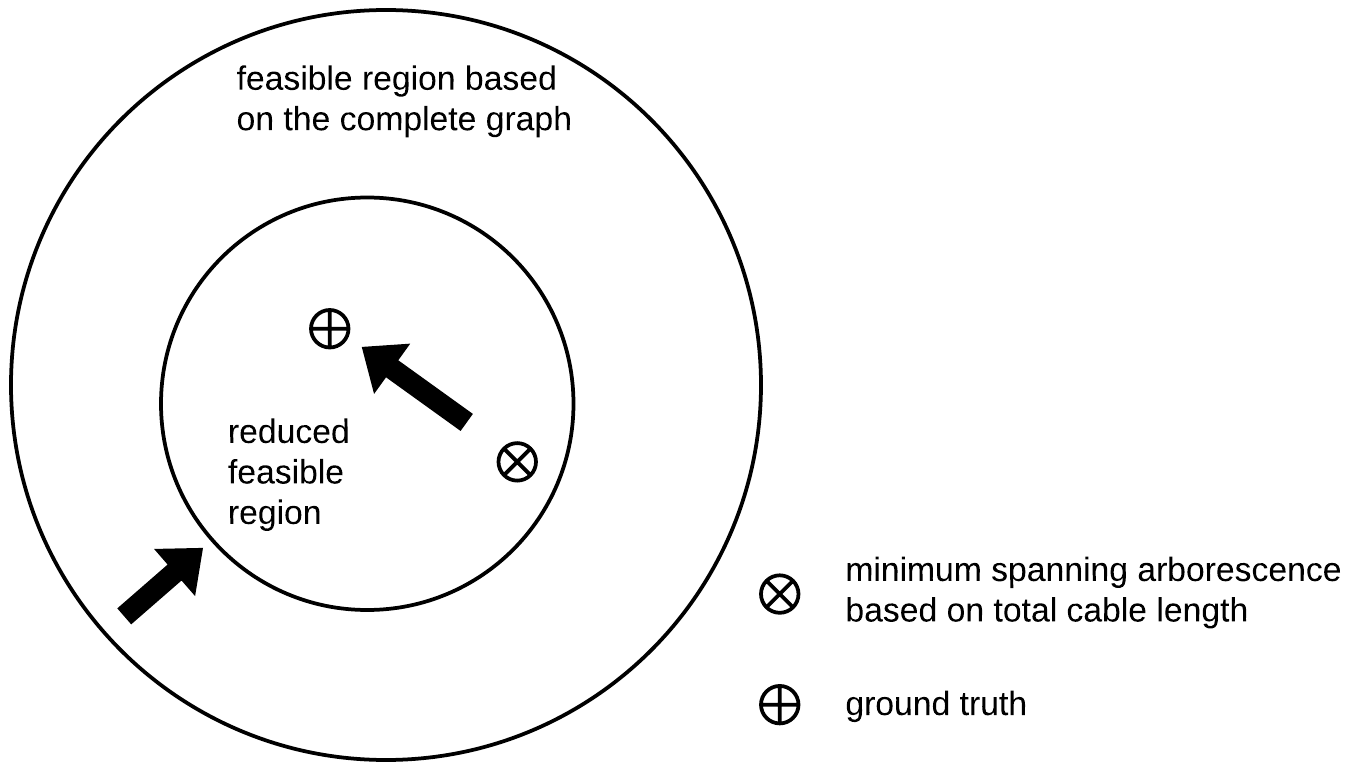
\includegraphics[width=0.7\linewidth]{Pictures/figFeasibleRegion} \end{center}

Combinatorial optimisation problem.

A \textbf{local search heuristic algorithm} is proposed to to move from \(\bigotimes\)
to \(\bigoplus\). \citep{michiels2007theoretical}

\begin{quote}
All the algorithms in this category have two parts, an objective funciton to
assess candidates and an neighbourhood function to generate candidates
systematically. Here, pseudo linearised power flow will be used as the
objective function and resuted mean squared error is to be minimised. It will
be discussed later. An algorithm to rank spanning arborescences according to
their total cable lengths is implemented.
\end{quote}

\begin{table}[H]
\centering
\begin{tabular}[t]{l|l|l}
\hline
function & what it does & in this project\\
\hline
objective & assess candidate & pseudo linearised power flow\\
\hline
neighbourhood & generate candidate & rank spanning arborescence\\
\hline
\end{tabular}
\end{table}

\begin{itemize}
\tightlist
\item
  Starting point -\textgreater{} minimum spanning arborescence
\item
  Every candidate is reachable.
\item
  Ground truth should be found before long.
\item
  Not in parallel.
\end{itemize}

\begin{quote}
Because power grids are to be built with less cost, the total cable length
of ground truth should not be too long, so we can find it before long,
\end{quote}

\hypertarget{ac-power-flow}{%
\chapter{AC Power Flow}\label{ac-power-flow}}

\begin{itemize}
\tightlist
\item
  two essential matrices \protect\hyperlink{matrices}{-\textgreater{} 4.1}
\item
  bus impedance matrix \protect\hyperlink{BIM}{-\textgreater{} 4.2}
\item
  direct impedance method for power flow calculation \protect\hyperlink{power-flow}{-\textgreater{} 4.2}
\end{itemize}

\begin{center}\rule{0.5\linewidth}{0.5pt}\end{center}

Can be generalised for multi-phase model. \citep{hsieh2017matrix}

\hypertarget{matrices}{%
\section{Two Matrices}\label{matrices}}

Current injection to flow:
\[
  \bar{\boldsymbol{I}}_{\text{edge}} =
  - \boldsymbol{K} \bar{\boldsymbol{I}}
\]

where \textbf{edge path incidence matrix (EPI)}, \(\boldsymbol{K}\).

Voltage drop to nodal voltage:
\[
  \bar{\boldsymbol{V}} =
  \bar{\boldsymbol{V}}_{\text{zero}}
  - \boldsymbol{K}^{\top} \boldsymbol{\bar{Z}}_\text{edge}
  \bar{\boldsymbol{I}}_{\text{edge}} 
\]

where \textbf{edge impedance diagonal block matrix (EIDB)},
\(\boldsymbol{\bar{Z}}_\text{edge}\).

\begin{center}\rule{0.5\linewidth}{0.5pt}\end{center}

\begin{center}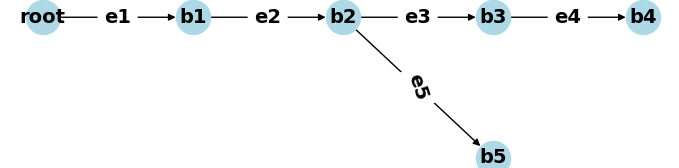
\includegraphics[width=0.7\linewidth]{Pictures/figCaseSix} \end{center}

\[ \begin{aligned}
    \left[\begin{array}{l}
    \bar{I}_{\text{edge}, 1} \\
    \bar{I}_{\text{edge}, 2} \\
    \bar{I}_{\text{edge}, 3} \\
    \bar{I}_{\text{edge}, 4} \\
    \bar{I}_{\text{edge}, 5}
    \end{array}\right]
    = - \left[\begin{array}{lllll}
    1 & 1 & 1 & 1 & 1 \\
    0 & 1 & 1 & 1 & 1 \\
    0 & 0 & 1 & 1 & 0 \\
    0 & 0 & 0 & 1 & 0 \\
    0 & 0 & 0 & 0 & 1
    \end{array}\right]
    \left[\begin{array}{l}
    \bar{I}_{1} \\
    \bar{I}_{2} \\
    \bar{I}_{3} \\
    \bar{I}_{4} \\
    \bar{I}_{5}
    \end{array}\right]
\end{aligned} \]

\[ \begin{aligned}
  &
  \left[\begin{array}{c}
    \bar{V}_{1} \\
    \bar{V}_{2} \\
    \bar{V}_{3} \\
    \bar{V}_{4} \\
    \bar{V}_{5}
  \end{array}\right]
  -
  \left[\begin{array}{c}
    \bar{V}_\text{rate} \\
    \bar{V}_\text{rate} \\
    \bar{V}_\text{rate} \\
    \bar{V}_\text{rate} \\
    \bar{V}_\text{rate}
  \end{array}\right]
  =
  - \left[\begin{array}{ccccc}
    1 & 1 & 1 & 1 & 1 \\ 
    0 & 1 & 1 & 1 & 1 \\ 
    0 & 0 & 1 & 1 & 0 \\ 
    0 & 0 & 0 & 1 & 0 \\ 
    0 & 0 & 0 & 0 & 1
  \end{array} \right]^{\top}
  \left[\begin{array}{ccccc}
    Z_{\text{edge}, 1} & 0 & 0 & 0 & 0 \\
    0 & Z_{\text{edge}, 2} & 0 & 0 & 0 \\
    0 & 0 & Z_{\text{edge}, 3} & 0 & 0 \\
    0 & 0 & 0 & Z_{\text{edge}, 4} & 0 \\
    0 & 0 & 0 & 0 & Z_{\text{edge}, 5}
  \end{array}\right]
  \left[\begin{array}{l}
    \bar{I}_{\text{edge}, 1} \\
    \bar{I}_{\text{edge}, 2} \\
    \bar{I}_{\text{edge}, 3} \\
    \bar{I}_{\text{edge}, 4} \\
    \bar{I}_{\text{edge}, 5}
  \end{array} \right]
\end{aligned} \]

\begin{center}\rule{0.5\linewidth}{0.5pt}\end{center}

Alternating current power flow: \citep{conti2006voltage}
\[
  \bar{\boldsymbol{V}} = \bar{\boldsymbol{V}}_{\text{zero}}
    + \left( \boldsymbol{K}^{\top} \boldsymbol{\bar{Z}}_\text{edge}
    \boldsymbol{K} \right) \bar{\boldsymbol{I}}
\]

\hypertarget{BIM}{%
\section{Bus Impedance Matrix}\label{BIM}}

Alternating current power flow:
\[
  \bar{\boldsymbol{V}} = \bar{\boldsymbol{V}}_{\text{zero}}
    + \left( \boldsymbol{K}^{\top} \boldsymbol{\bar{Z}}_\text{edge}
    \boldsymbol{K} \right) \bar{\boldsymbol{I}}
\]

\begin{center}\rule{0.5\linewidth}{0.5pt}\end{center}

\textbf{Bus impedance matrix (BIM)}, \(\boldsymbol{\bar{Z}}\), is defined as:
\[ \begin{aligned}
  \boldsymbol{\bar{Z}}
    &= \boldsymbol{K}^{\top} \boldsymbol{\bar{Z}}_\text{edge}
    \boldsymbol{K} \\
    &= \boldsymbol{R} + j \boldsymbol{X}
\end{aligned} \]

where \textbf{bus resistance matrix (BRM)}, \(\boldsymbol{R}\): real part of entries
in BIM.

\hypertarget{power-flow}{%
\section{Direct Impedance Method}\label{power-flow}}

Build BIM directly and calculate power flow. \citep{schneider2017analytic}

Five steps to build BIM:

\begin{enumerate}
\def\labelenumi{\arabic{enumi}.}
\tightlist
\item
  Define a unit impedance matrix.
\item
  Calculate edge impedance matrices for cables.
\item
  Build EIDB.
\item
  Obtain EPI based on topology.
\item
  Calculate BIM using EIDB and EPI.
\end{enumerate}

\hypertarget{fixed-point-method}{%
\subsection*{Fixed Point Method}\label{fixed-point-method}}
\addcontentsline{toc}{subsection}{Fixed Point Method}

To calculate power flow in one snapshot, given power injections, the following
procedure is repeated:
\[ \begin{aligned}
    \boldsymbol{\bar{I}} &= \boldsymbol{\underline{P}}
      \otimes \boldsymbol{\underline{V}}_\text{previous} \\
    \boldsymbol{\bar{V}}
    &= \boldsymbol{\bar{Z}} \boldsymbol{\bar{I}}
      + \boldsymbol{\bar{V}}_\text{zero} \\
    \epsilon
    &= \left( \boldsymbol{\bar{V}} - \boldsymbol{\bar{V}} \right)^\top
      \left( \boldsymbol{\bar{V}} - \boldsymbol{\bar{V}} \right)
\end{aligned} \]
until \(\epsilon\) is smaller than a pre-defined threshold.

\hypertarget{linearised-power-flow}{%
\chapter{Linearised Power Flow}\label{linearised-power-flow}}

Two steps:

\begin{itemize}
\tightlist
\item
  linearise voltage drop \protect\hyperlink{linearVoltageDrop}{-\textgreater{} 5.1}
\item
  ignore power loss \protect\hyperlink{linearVoltage}{-\textgreater{} 5.2}
\end{itemize}

Then:

\begin{itemize}
\tightlist
\item
  assessment of candidate \protect\hyperlink{assessment}{-\textgreater{} 5.5}
\end{itemize}

\begin{center}\rule{0.5\linewidth}{0.5pt}\end{center}

\begin{itemize}
\tightlist
\item
  bus resistance matrix \protect\hyperlink{BRM}{-\textgreater{} 5.3}
\item
  inversed bus resistance matrix \protect\hyperlink{brmInv}{-\textgreater{} 5.4}
\item
  error from linearisation \protect\hyperlink{error}{-\textgreater{} 5.6}
\end{itemize}

\hypertarget{linearVoltageDrop}{%
\section{Linearised Voltage Drop}\label{linearVoltageDrop}}

With power flow at source of edge \(k\), \(\bar{S}_{\text{source}, k}\):
\[
\bar{I}_{\text{edge}, k}
  = \frac{\underline{S}_{\text{source}, k}}{\underline{V}_i} \\
\]

Voltage drop:
\[
\begin{aligned}
  \bar{V}_{\text{edge}, k}
  &= \bar{I}_{\text{edge}, k} \bar{Z}_{\text{edge}, k} \\
  &= \frac{
    \underline{S}_{\text{source}, k} \bar{Z}_{\text{edge}, k}
  }{\underline{V}_i} \\
  &= \frac{
    \left(P_{\text{source}, k} - j Q_{\text{source}, k} \right)
    \left(R_{\text{edge}, k} + j X_{\text{edge}, k} \right)
  }{\underline{V}_i} \\
  &= \frac{
    R_{\text{edge}, k} P_{\text{source}, k}
    + X_{\text{edge}, k} Q_{\text{source}, k}
  }{\underline{V}_i}
  + j \frac{
    X_{\text{edge}, k} P_{\text{source}, k}
    - R_{\text{edge}, k} Q_{\text{source}, k}
  }{\underline{V}_i}
\end{aligned}
\]

Then: \citep{conti2006voltage}
\[
V_{\text{edge}, k} =
  \frac{R_{\text{edge}, k}}{V_\text{rate}} P_{\text{source}, k}
\]

\begin{itemize}
\tightlist
\item
  Ignore imaginary part.
\item
  Replace \(\underline{V}_i\) with \(V_\text{rate}\).
\end{itemize}

\hypertarget{linearVoltage}{%
\section{Linearised Voltage}\label{linearVoltage}}

Voltage drop to nodal voltage:
\[
\boldsymbol{V}
  = \boldsymbol{V}_\text{zero}
  - \frac{1}{V_\text{rate}} \boldsymbol{K}^{\top}
  \boldsymbol{R}_\text{edge} \boldsymbol{P}_\text{source}
\]

Power injection to flow:
\[
\boldsymbol{P}_\text{source}
  = - \boldsymbol{K}
  \left(\boldsymbol{P} - \boldsymbol{P}_\text{loss} \right)
\]

\begin{center}\rule{0.5\linewidth}{0.5pt}\end{center}

Voltage magnitude can be calculated using BRM and real power injections:
\[ \begin{aligned}
  \boldsymbol{V} &= \boldsymbol{V}_\text{zero} + \frac{1}{V_\text{rate}}
    \left(
      \boldsymbol{K}^{\top} \boldsymbol{R}_\text{edge} \boldsymbol{K}
    \right) \boldsymbol{P} \\
  {} &= \boldsymbol{V}_\text{zero}
      + \frac{1}{V_\text{rate}} \boldsymbol{R} \boldsymbol{P}
\end{aligned} \]

\begin{itemize}
\tightlist
\item
  To \protect\hyperlink{assessment}{assess candidate} by calculating power injection using
  voltage magnitudes.
\end{itemize}

\hypertarget{BRM}{%
\section{Bus Resistance Matrix}\label{BRM}}

\begin{itemize}
\tightlist
\item
  Bus 2 -\textgreater{} root
\item
  69 PQ buses
\item
  207 channels
\item
  207 rows and 207 columns
\end{itemize}

\begin{center}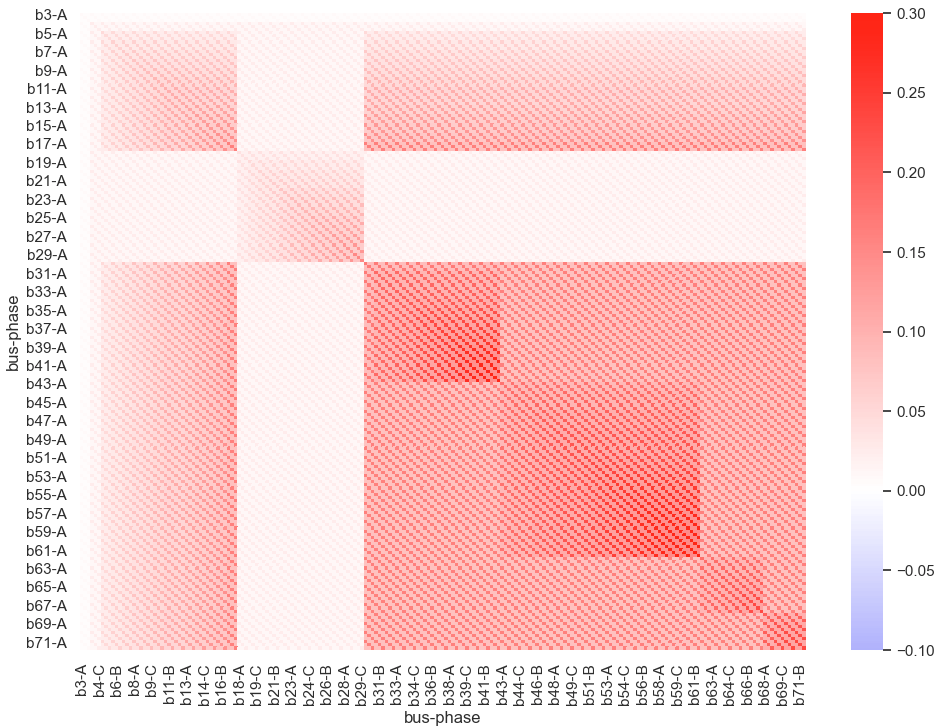
\includegraphics{Pictures/figHeatmapBRM} \end{center}

\begin{quote}
There is some pattern that can be explained by the analytical expression for
entries in BRM.
\end{quote}

\hypertarget{LCA}{%
\subsection*{Lowest Common Ancestor Problem}\label{LCA}}
\addcontentsline{toc}{subsection}{Lowest Common Ancestor Problem}

Entry \((i, j)\) -\textgreater{} sum of edge resistances in their common path to root:
\[
R_{i, j}=\sum_{k \in U_{i} \cap U_{j}} R_{\text {edge }, k}
\]
where \(U_{i}\) is set of edges on the path from root to bus \(i\).

\begin{quote}
Entry \((i, j)\) is the sum of edge resistances in the path from root to their
lowest common ancestor (LCA) of bus \(i\) and \(j\).
\end{quote}

\begin{itemize}
\tightlist
\item
  Calcualted efficiently using LCA for all pairs.
\item
  Useful pattern.
\end{itemize}

\begin{quote}
BRM can be calcualted efficiently using LCA for all pairs of buses. and the
pattern can be used in future work.
\end{quote}

For example,

\begin{center}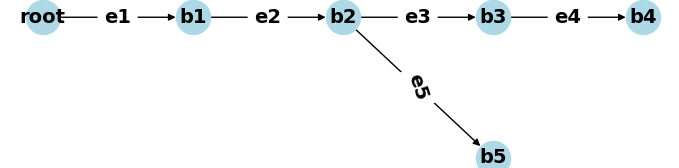
\includegraphics[width=0.7\linewidth]{Pictures/figCaseSix} \end{center}

\[ \begin{array}{ll}
  \hline
  \text{pair of buses} & \text{entry in BRM} \\
  \hline
  \text{b3-b5} & R_\text{e1} + R_\text{e2} \\
  \text{b4-b5} & R_\text{e1} + R_\text{e2} \\
  \hline
\end{array} \]

\begin{center}\rule{0.5\linewidth}{0.5pt}\end{center}

\protect\hyperlink{summary}{-\textgreater{} summary}

\hypertarget{brmInv}{%
\section{Pseudo Linearised Power Flow}\label{brmInv}}

Based on linearised power flow, \(\boldsymbol{V} = \boldsymbol{V}_\text{zero} + \frac{1}{V_\text{rate}} \boldsymbol{R} \boldsymbol{P}\):
\[ \begin{aligned}
    \boldsymbol{P}_\text{assess} =
    V_\text{rate} \boldsymbol{R}^{\top}
    \left( \boldsymbol{V} - \boldsymbol{V}_\text{zero} \right)
\end{aligned} \]
-\textgreater{} \textbf{pseudo linearised power flow}.

\begin{quote}
which is referred to as pseudo linearised power flow.
\end{quote}

Inversed BRM for case-70:

\begin{quote}
Inversed BRM for the case looks like:
\end{quote}

\begin{center}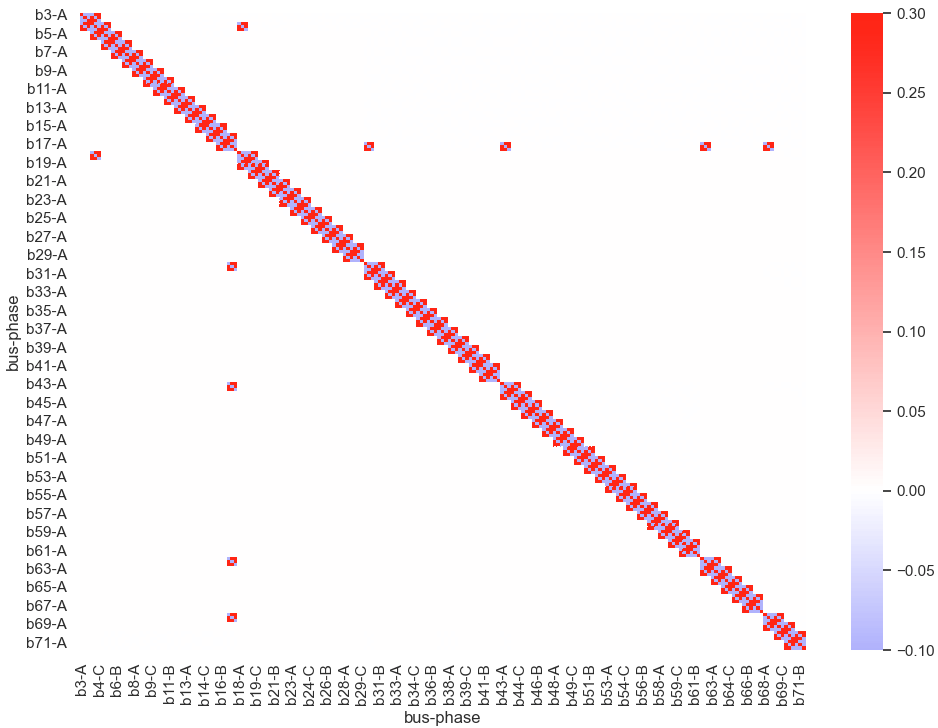
\includegraphics{Pictures/figHeatmapBrmInv} \end{center}

\begin{itemize}
\tightlist
\item
  Sparse.
\item
  Full rank.
\item
  Voltage magnitude at any channel can have a huge impact.
\item
  Useful pattern.
\end{itemize}

\hypertarget{assessment}{%
\section{Assessment of Candidate}\label{assessment}}

\begin{itemize}
\tightlist
\item
  Calculate \(\boldsymbol{P}_\text{assess}\) using voltage magnitudes.
\item
  Compare \(\boldsymbol{P}_\text{assess}\) with available power measurements.
\end{itemize}

\textbf{Mean squared error (MSE)}:
\[ \begin{aligned}
  \mathcal{H}(\boldsymbol{R}) =
  \left[
    (\boldsymbol{P}_\text{assess} - \boldsymbol{P})
    \otimes \boldsymbol{O}
  \right]^\top
  \cdot \left[
    (\boldsymbol{P}_\text{assess} - \boldsymbol{P})
    \otimes \boldsymbol{O}
  \right]
  / |\mathcal{O}|
\end{aligned} \]
where:

\begin{itemize}
\tightlist
\item
  \(\mathcal{O}\): set of observed active channels and inactive channels.
\item
  \(\boldsymbol{O}\): binary vector indicating observed active channels.
\end{itemize}

\begin{quote}
It is the second term in the objective function. Entries for unobserved
active channels are ignored.
\end{quote}

\hypertarget{error}{%
\section{Error from Linearisation}\label{error}}

Box plot:

\begin{itemize}
\tightlist
\item
  with respect to different number of observed active channels
\item
  based on ground truth and 50 snapshots\footnote{during 00:00:00 and 00:00:50 on Dec
    2, 2020 from Sonnen data set.}
\end{itemize}

\begin{center}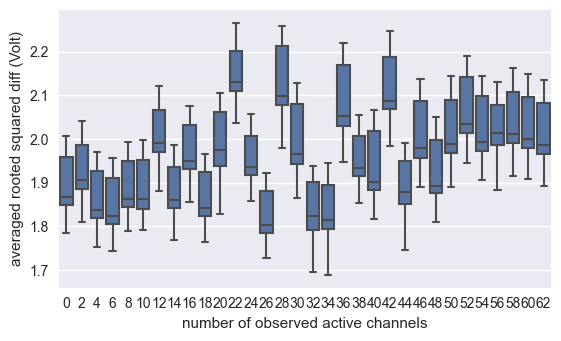
\includegraphics{Pictures/figErrorObsBRM} \end{center}

\begin{itemize}
\tightlist
\item
  Error is aleady reduced to 1.7 \textasciitilde{} 2.2.
\item
  Rated voltage magnitudes will increase the error dramatically.
\end{itemize}

\begin{quote}
Rated voltage magnitudes will increase the error dramatically, so full
observability of voltage magnitudes are still required for now.
\end{quote}

\protect\hyperlink{summary}{-\textgreater{} summary}

\hypertarget{result-and-discussion}{%
\chapter{Result and Discussion}\label{result-and-discussion}}

\begin{itemize}
\tightlist
\item
  result for case-70 \protect\hyperlink{result}{-\textgreater{} 6.1}
\item
  summary \protect\hyperlink{summary}{-\textgreater{} 6.2}
\end{itemize}

\hypertarget{result}{%
\section{Result for Case-70}\label{result}}

\begin{itemize}
\tightlist
\item
  three new pairs, ``b29‐b44'', ``b68‐b14'', and ``b68‐b15''
\item
  144 edges in total
\item
  288 SAs rooted at ``b2''
\end{itemize}

\begin{center}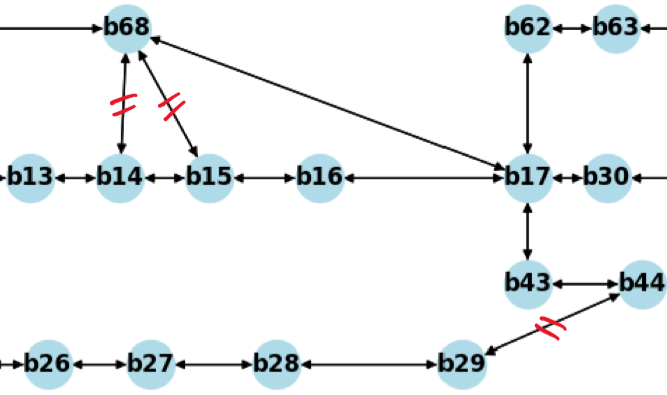
\includegraphics[width=0.55\linewidth]{Pictures/case70} \end{center}

Rank SAs according to total cable lengths:

\begin{center}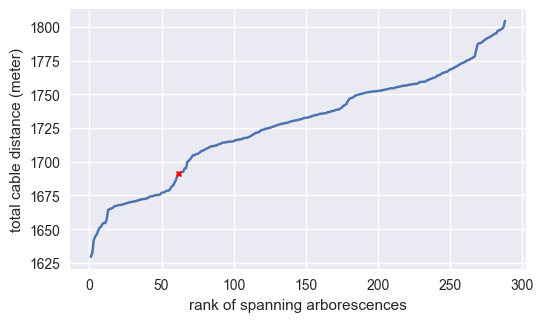
\includegraphics{Pictures/distances_288} \end{center}

\begin{quote}
Total cable length increases all the time. That is, we rank spanning
arborescences according to their total cable lengths.
\end{quote}

Assessment based on 50 snapshots\footnote{during 00:00:00 and 00:00:50 on Dec 2, 2020
  from Sonnen data set.}:

\begin{center}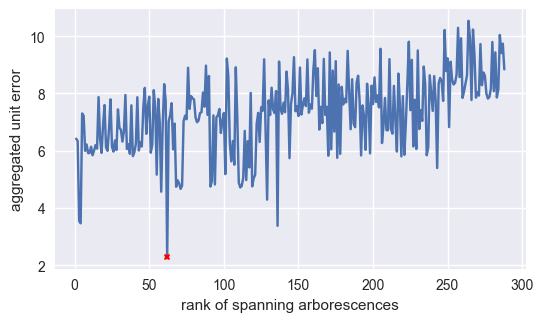
\includegraphics{Pictures/errors_288} \end{center}

\hypertarget{summary}{%
\section{Summary}\label{summary}}

\begin{itemize}
\tightlist
\item
  Topology inference -\textgreater{} combinatorial optimisation problem.
\item
  A framework is proposed.
\item
  Core: local search heuristic algorithm.
\end{itemize}

Advantages:

\begin{itemize}
\tightlist
\item
  Robust to partial observability.
\item
  Integrate all kinds of information in weight and direction.
\end{itemize}

Four steps:

\begin{enumerate}
\def\labelenumi{\arabic{enumi}.}
\tightlist
\item
  Shrink feasible region (reduce number of SAs).
\item
  Measure the size of feasible region by counting number of SAs.
\item
  Get candidates sequentially by ranking SAs according to total cable lengths.
\item
  Assess candidates based on available measurements.
\end{enumerate}

\hypertarget{issues}{%
\subsection*{Issues}\label{issues}}
\addcontentsline{toc}{subsection}{Issues}

\begin{enumerate}
\def\labelenumi{\arabic{enumi}.}
\tightlist
\item
  Too many spanning arborescences. (\protect\hyperlink{overlapping}{remove overlapping edges})
\item
  Full observability over voltage magnitudes. (\protect\hyperlink{BRM}{matrices with full
  rank})
\item
  Error in linearised power flow calculation. (\protect\hyperlink{error}{error from
  linearisation})
\end{enumerate}

\hypertarget{future-work}{%
\subsection*{Future Work}\label{future-work}}
\addcontentsline{toc}{subsection}{Future Work}

\begin{itemize}
\tightlist
\item
  How to detect more impossible potential edges. (for issue 1)
\item
  How to assess candidates based on a fraction. (for issue 2)
\item
  How to use voltage sensitivity matrix in linearised power flow. (for issue 3)
\end{itemize}

  \bibliography{bibliography.bib}

\end{document}
